\documentclass[11pt,a4paper]{article}
\usepackage[margin=2.5cm]{geometry}
\usepackage[T1]{fontenc}
\usepackage{lmodern}
\usepackage{microtype}
\usepackage[authoryear,round]{natbib}
\usepackage[hidelinks]{hyperref}
\usepackage{enumitem}
\usepackage{tikz}
\usetikzlibrary{positioning,arrows.meta,calc,fit}
\setlist{itemsep=2pt,topsep=4pt}

\title{Understanding Data Scarcity in Foundation-Model-Based\\Histopathology Patch Classification}
\author{Yannik Queisler\\[2pt]\small Thesis Proposal}
\date{\today}

\begin{document}
\maketitle

\section{Motivation}
Pathology foundation models, pretrained with self-supervision on large slide collections, have become the default way to represent histopathology patches \citep{chen2024uni,vorontsov2024virchow}.
Public models are now compared systematically on clinical tasks \citep{campanella2025benchmark}, yet such benchmarks vary the model and fix the downstream data.
How much labelled data a classifier on top of these representations needs is much less understood, although labels are expensive \citep{lu2021dataEfficient} and thinnest for the rare cancers these models are promoted for \citep{vorontsov2024virchow}.

Nominal sample counts are a poor measure of data sufficiency.
Patches are nested within patients, and mixing them across training and evaluation inflates reported scores by up to 41\% \citep{bussola2021leakage}; thousands of patches may carry the information of a few dozen patients.
Class frequencies are also strongly uneven, which in medical imaging distorts both discrimination and calibration \citep{mosquera2024classImbalance}, and long-tailed recognition work separates representation from classifier training \citep{kang2020decouplingRepresentation}.
With frozen features the representation is fixed, so the imbalance effect can be studied on the classifier alone.
Clinical use also needs well-calibrated probabilities, which modern networks often lack \citep{guo2017calibration}.

This thesis therefore separates three forms of scarcity: skewed class allocation, too few patches, and too few patients.
It asks which of them drives the performance loss of classifiers trained on foundation-model representations, why, and how far algorithms can compensate, telling practitioners where annotation effort pays off and when a better algorithm cannot replace it.

\section{Research Questions}
\begin{enumerate}
  \item \textbf{Class imbalance.} How does it affect discrimination and calibration, and which mechanisms cause the loss?
  \item \textbf{Patch shortage.} How does it affect performance when patient coverage is held constant?
  \item \textbf{Patient shortage.} How does it affect performance independently of patch count, and which properties of the learned feature distributions explain the loss?
  \item \textbf{Mitigation.} Which forms of scarcity can be mitigated algorithmically without acquiring more data?
\end{enumerate}

\section{Methodology}
Controlled experiments use TCGA-UT \citep{komura2022universalEncoding} (patches from 32 cancer types) and BRACS \citep{brancati2022bracs} (breast lesions including atypical categories) with frozen pathology foundation-model representations.
Three factors are manipulated separately while the others are controlled (Figure~\ref{fig:design}):
\begin{itemize}
  \item \textbf{Class allocation:} how the training data is distributed across classes.
  \item \textbf{Patch count:} patches per patient, with patient coverage held constant.
  \item \textbf{Patient count:} number of independent patients, with patch count held constant.
\end{itemize}

\begin{figure}[ht]
  \centering
  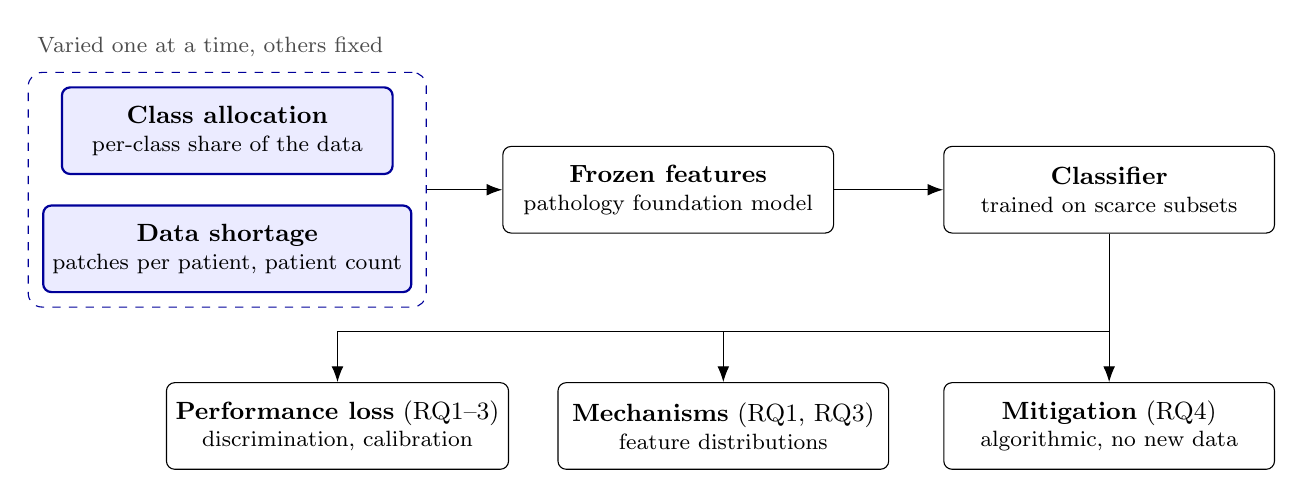
\begin{tikzpicture}[
      font=\small,
      box/.style={draw, rounded corners=3pt, minimum width=4.2cm, minimum height=1.1cm, align=center},
      var/.style={box, fill=blue!8, draw=blue!60!black, thick},
      arr/.style={-{Latex[length=2mm]}}]
    \node[var] (c) at (0,0.75) {\textbf{Class allocation}\\[-1pt]{\footnotesize per-class share of the data}};
    \node[var] (d) at (0,-0.75) {\textbf{Data shortage}\\[-1pt]{\footnotesize patches per patient, patient count}};
    \node[draw=blue!60!black, dashed, rounded corners=5pt, inner sep=5pt, fit=(c)(d)] (fac) {};
    \node[box] (f) at (5.6,0) {\textbf{Frozen features}\\[-1pt]{\footnotesize pathology foundation model}};
    \node[box] (k) at (11.2,0) {\textbf{Classifier}\\[-1pt]{\footnotesize trained on scarce subsets}};
    \node[box] (l) at (1.4,-3.0) {\textbf{Performance loss} (RQ1--3)\\[-1pt]{\footnotesize discrimination, calibration}};
    \node[box] (m) at (6.3,-3.0) {\textbf{Mechanisms} (RQ1, RQ3)\\[-1pt]{\footnotesize feature distributions}};
    \node[box] (g) at (11.2,-3.0) {\textbf{Mitigation} (RQ4)\\[-1pt]{\footnotesize algorithmic, no new data}};
    \node[above=2pt of fac.north west, anchor=south west, font=\footnotesize, text=black!70] {Varied one at a time, others fixed};
    \draw[arr] (fac.east) -- (f.west);
    \draw[arr] (f.east) -- (k.west);
    \draw (k.south) -- (11.2,-1.8);
    \draw (1.4,-1.8) -- (11.2,-1.8);
    \draw[arr] (1.4,-1.8) -- (l.north);
    \draw[arr] (6.3,-1.8) -- (m.north);
    \draw[arr] (11.2,-1.8) -- (g.north);
  \end{tikzpicture}
  \caption{Experimental design. Each scarcity factor (blue) is varied alone while the others stay fixed.}
  \label{fig:design}
\end{figure}

Every setting is scored on discrimination and calibration.
Mechanism analyses look at class influence, tail support and how well class-level patient distributions are estimated in feature space.
Representative mitigation approaches are then tested against the loss each factor causes.

\section{Preliminary Findings}
First experiments show that class imbalance costs frozen-feature probes little on TCGA-UT at first and then accelerates (balanced-accuracy loss 0.6\,pp at a largest-to-smallest class ratio of 10, 2.9\,pp at 100), but starts immediately and is 2.6 times larger on BRACS (7.7\,pp at 100).
Unequal class influence and reduced tail support both contribute and compound at high ratios.
Calibration error rises, but one global temperature removes 92--96\% of the increase.
Patient shortage produces a distinct loss, caused mainly by poor estimation of class-level patient distributions, and increasing patch depth cannot fully substitute for patient breadth.
Mitigation of patient-shortage damage has so far been limited.

\section{Expected Contribution}
The thesis gives a systematic account of how \textbf{class allocation, patch support and patient support} contribute differently to data scarcity in computational pathology.
The resulting framework should clarify three things:
\begin{itemize}
  \item when additional nominal samples help,
  \item when independent patient diversity matters more,
  \item when algorithmic mitigation can compensate for limited data.
\end{itemize}


\clearpage
\bibliographystyle{plainnat}
\bibliography{references}

\end{document}
